\documentclass[11pt]{article}

\def\articlename{统计整理}
\def\authorname{杨弘毅}
\def\startdate{2020年4月9日}

\ifx \authorname\undefined
  \def\authorname{杨弘毅}
\else
\fi

\author{\authorname}
\date{创建:\startdate \\修改:\today}

\usepackage[a4paper,left=6em,right=6em]{geometry}
\usepackage{amsmath,amsfonts,amsthm,bbold}
\usepackage{booktabs,float,multirow}
\usepackage{cancel}
\usepackage{enumitem}
\usepackage{multicol}
\usepackage{graphicx}
\usepackage[toc,title]{appendix}
\usepackage{tikz}
\usetikzlibrary{arrows.meta}
\usetikzlibrary{patterns}
\usetikzlibrary{decorations.pathreplacing}
\usetikzlibrary{decorations.pathmorphing}
\usepackage{subcaption}
\usepackage{fancyhdr}
\pagestyle{fancy}
\setlength{\headheight}{15pt}
\usepackage{footmisc}
\usepackage{hyperref}
\usepackage{tocloft}
\hypersetup{
    colorlinks=true, %set true if you want colored links
    linkcolor=blue,
    linktoc=all, %set to all if you want both sections and subsections linked
    citecolor=black,
    filecolor=black,
    urlcolor=blue
}
\usepackage[UTF8]{ctex}

\title{\articlename}

% Format
\setlength{\cftbeforesecskip}{6pt}
\setlength{\parskip}{0.6em}
\renewcommand{\baselinestretch}{1.4}
\setlist{noitemsep,itemindent=1em,topsep=0em,leftmargin=4em,rightmargin=4em}
\setlist[2]{leftmargin=2em}

% Shortcut
\newcommand{\divider}{\vspace{-\parskip}\noindent\rule{\linewidth}{0.4pt}}
\newcommand{\tops}[1]{\texorpdfstring{#1}{TEXT}}

% Theorem
\newtheorem{thm}{定理}[section] 
\newtheorem{proposition}[thm]{命题}
\newtheorem{lemma}[thm]{引理}
\newtheorem{corollary}[thm]{推论}
\newtheorem{property}[thm]{性质}
\newtheorem{example}[thm]{例子}
\newtheorem{remark}[thm]{备注}
\newtheorem{note}[thm]{注释}

% Symbol
\newcommand{\E}{\mathbb{E}}
\newcommand{\mcl}{\mathcal{L}}
\newcommand{\rnE}{\widetilde{\mathbb{E}}}
\newcommand{\wt}[1]{\widetilde{#1}}
\DeclareMathOperator{\Var}{Var}
\DeclareMathOperator{\Cov}{Cov}
\newcommand{\abs}[1]{\left\lvert #1\right\rvert}
\newcommand{\norm}[1]{\left\lVert #1\right\rVert}
\newcommand{\given}{\:\vert\:}

\begin{document}
\maketitle
\tableofcontents

\section{TODO}
\begin{itemize}
    \item 参数与非参数方法
    \item conditional probability projection
    \item likelihood, log-likelihood, goodness-of-fit, quasi-maximum likelihood, ratio test
    \item Chi-square, joint hypothesis
    \item Newey West 1987
    \item Durbin Watson
\end{itemize}

\section{基础}

\subsection{期望}

对于随机变量$X$,其概率空间为$(\Omega,\mathcal{F},P)$,期望值$\E[X]$,应有:
\begin{equation*}
    \E[X] = \int_{\Omega} X(\omega) dP(\omega)
\end{equation*}

在离散以及连续情形下有如下定义,其中$f(x)$为变量$X$的概率密度函数(PDF)。
\begin{align*}
    \E[X] &= \sum_{i=i}^n x_i p_i =x_1 p_1 + x_2 p_2 + \dots + x_n p_n \\
    \E[X] &= \int x f(x) dx
\end{align*}

其性质有:
\begin{align*}
    \E[X+Y] &= \E[X] + \E[Y] \\
    \E[aX] &= a \E[X] \\
    \E[XY] &= \E[X]\E[Y] \quad \text{(X,Y are independent)}
\end{align*}

\subsection{方差}

对于方差(Variance),定义有:
\begin{align*}
    \Var(X) &= \Cov(X,X) = \sigma_X^2\\ 
    &= \E[(X-\E[X])^2] \\
    &= \E[X^2 - 2X\E[X] + \E[X]^2] \\
    &= \E[X^2] - 2\E[X]^2 + \E[X]^2 \\
    &= \E[X^2] - \E[X]^2
\end{align*}

其性质有:
\begin{align*}
    \Var(X + a) &= \Var(X) \\
    \Var(aX) &= a^2\Var(X) \\
    \Var(aX \pm bY) &= a^2\Var(X) + b^2\Var(Y) \pm 2ab \Cov(X,Y) \\
    \Var(\sum_{i=1}^{N} X_i) &= \sum_{i,j=1}^{N}\Cov(X_i,X_j) = \sum_{i=1}^{N}\Var(X_i) + \sum_{i \neq j}\Cov(X_i,X_j) \\
    \Var(\sum_{i=1}^{N} a_i X_i) &= \sum_{i,j=1}^{N}a_i a_j\Cov(X_i,X_j) \\
    &= \sum_{i=1}^{N}a_i^2\Var(X_i) + \sum_{i \neq j} a_i a_j \Cov(X_i,X_j) \\
    &= \sum_{i=1}^{N}a_i^2\Var(X_i) + 2\sum_{1 \leq i \leq j \leq N} a_i a_j \Cov(X_i,X_j)
\end{align*}

\subsection{协方差}

对于协方差(Covariance)其定义有:
\begin{align*}
    \Cov(X,Y) &= \E[(X-E(X))(Y-E(Y))] \\
    &= \E[XY - X\E[Y] -Y\E[X]+ \E[X]\E[Y]] \\
    &= \E[XY] - \E[X]\E[Y] - \E[X]\E[Y] + \E[X]\E[Y] \\
    &= \E[XY] - \E[X]\E[Y]
\end{align*}

性质有:
\begin{align*}
    \Cov(X,a) &= 0 \\
    \Cov(X,X) &= \Var(X) \\
    \Cov(X,Y) &= \Cov(Y,X) \\
    \Cov(aX,bY) &= ab\Cov(X,Y) \\
    \Cov(X+a,Y+b) &= \Cov(X,Y) \\
    \Cov(aX+bY,cW+dV) &= ac\Cov(X,W)+ad\Cov(X,V)+bc\Cov(Y,W)+bd\Cov(Y,V)
\end{align*}

\subsection{相关系数}

相关系数(Correlation Coefficient),为研究变量间线性相关程度的量。最早由统计学家卡尔·皮尔逊设计,也称为皮尔逊积矩相关系数(Pearson product-moment correlation coefficient),或皮尔逊相关系数:
\begin{equation*}
    \rho_{X,Y} = \frac{\Cov(X,Y)}{\sigma_X\sigma_Y}
    = \frac{\E[(X-\E[X])(Y-\E[Y])]}{\sigma_X\sigma_Y}
\end{equation*}

\section{矩}

\subsection{理解}

在物理学中,矩(Moment)源于阿基米德的杠杆原理,可简单认为是物理量与参照点距离的乘积。具体而言,$n$阶矩$\mu_n$为物理量$Q$与某参考点$r$的$n$次方的乘积,即$\mu_n = r^n Q$。常见的物理量如力或电荷等,若物理量并非集中在单点上,矩就应该是在物理量在空间上的积分,因有:$\mu_u = \int r^n \rho(r) dr$,其中$\rho(r)$为物理量的密度分布函数。


如力与力臂(参考点的距离)的乘积,得到的是力矩(或扭矩)。可以理解为一杆“秤”,“秤”的平衡的两边重量与距离的乘积相同,则能保持平衡。

而物理中的矩与数学中的矩概念相通,而在概率论上,可以理解秤为一杆秤的两端的概率为1,中心点概率为0。如一端秤砣重量,为中奖金额$500$元,但中奖概率为千分之一,即离中心点距离为$0.1\%$,那么期望为$0.5$元。可以理解为了使得秤保持平衡,则另一端,在概率为1,其秤砣重量,中奖金额应为$0.5$元。

\begin{figure}[ht!]
    \centering
    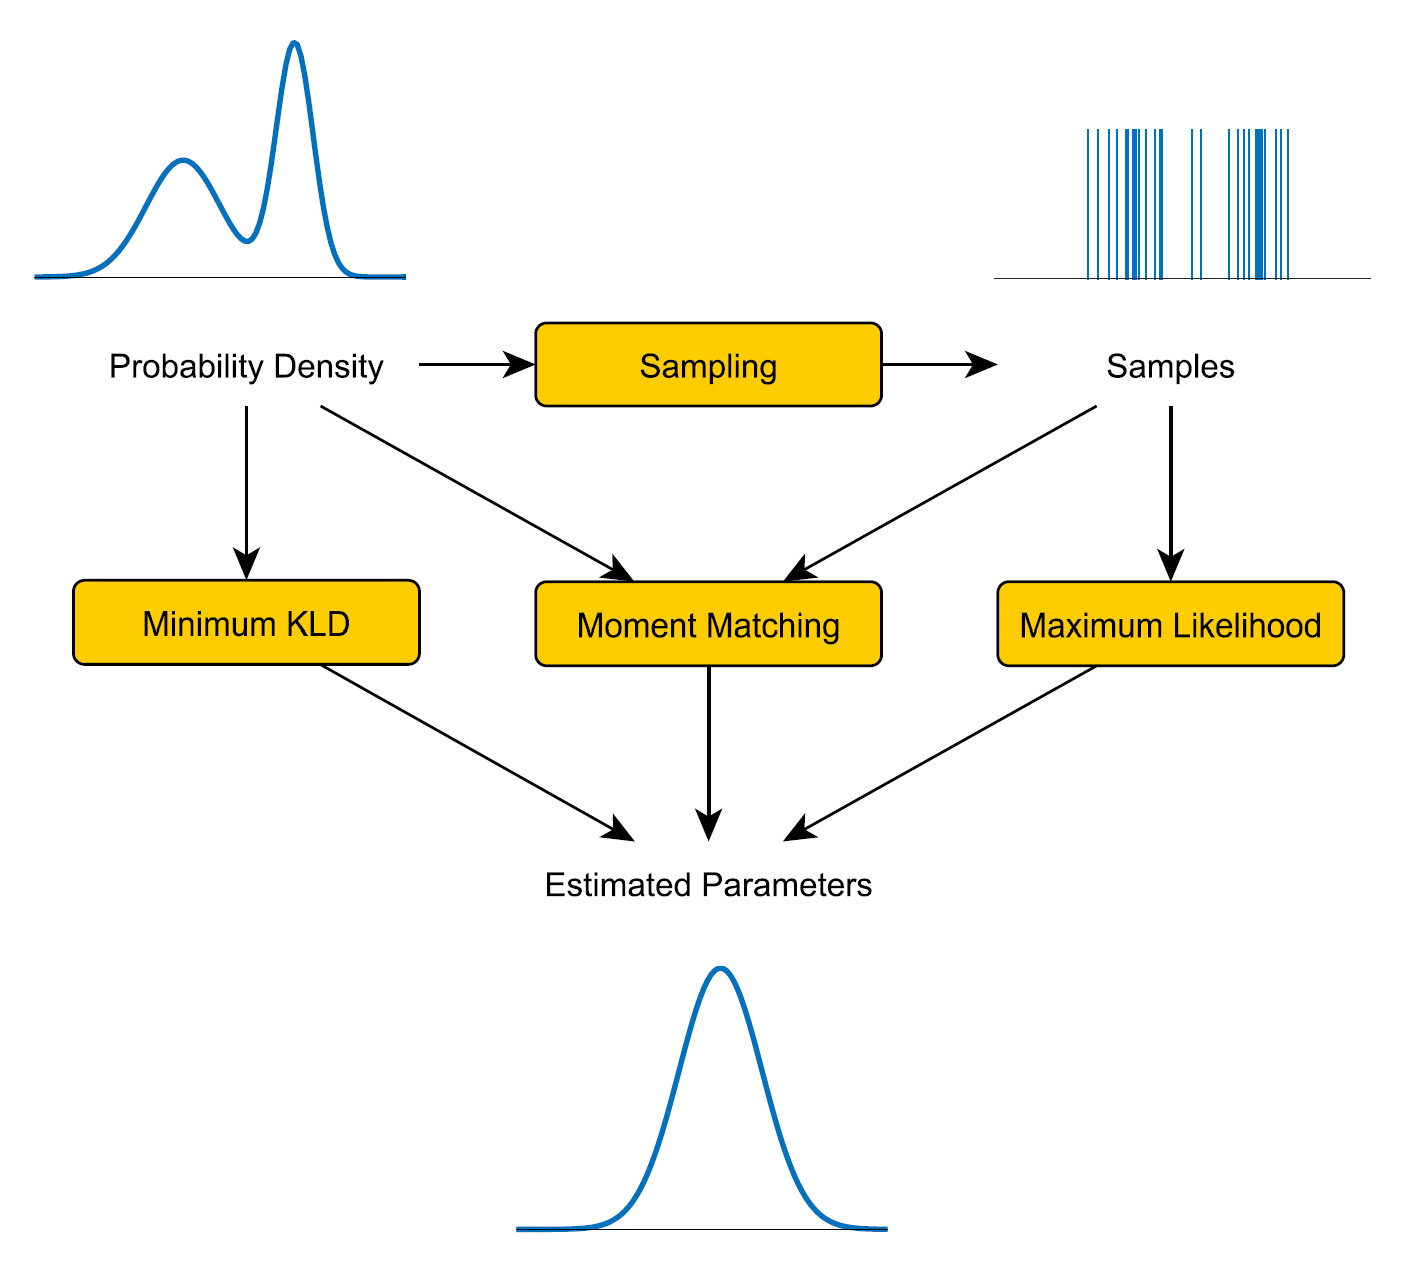
\includegraphics[width=0.6\textwidth]{fig/moment-matching.png}
    \caption{矩匹配}
    \label{fig:moment-match}
\end{figure}

\subsection{期望}

这样既可以把期望看成是矩,即距离(概率)乘以力(随机变量)的大小。对于$n$阶矩即对$x^n$q求期望,在离散形式下有:
\begin{equation*}
    E[x] = \sum_i p_i x_i
\end{equation*}

在连续形式下,n阶矩可以表示为$(x-c)^n$的期望,其中$f(x)$为概率密度函数(probability density function):
\begin{equation*}
    \mu_n = \int_{-\infty}^{\infty} (x-c)^n f(x) dx
\end{equation*}

\begin{table}[ht!]
\centering
\begin{tabular}{@{}cll@{}}
\toprule
阶(Order) & \multicolumn{1}{c}{非中心矩(Non-central)} & \multicolumn{1}{c}{中心矩(Central)} \\ \midrule
1st & $\E(x)=\mu $ & \\
2nd & $\E(x^2) $ & $\E[(x-\mu)^2]$   \\
3rd & $\E(x^3) $ & $\E[(x-\mu)^3]$   \\
4th & $\E(x^4) $ & $\E[(x-\mu)^4]$   \\ \bottomrule
\end{tabular}
\end{table}

常用的有一至四阶矩:
\begin{itemize}
    \setlength{\itemsep}{0em}
    \item 均值 $\text{Mean}(x)$ 为一阶中心矩
    \item 方差 $\text{Variance}(x) = \E(x-\mu)^2$ 为二阶非中心矩
    \item 偏度 $\text{Skewness}(x) = \frac{\E[(x-\mu)^4]}{\sigma^3}$ 为三阶标准矩 
    \item 峰度 $\text{Kurtosis}(x) = \frac{\E[(x-\mu)^4]}{\sigma^4}$ 为四阶标准矩
\end{itemize}

\subsection{分类}

\subsubsection*{原点矩(Raw/crude moment)}

当$c=0$时,称为原点矩。此时则有\textbf{平均数(mean)}或\textbf{期望(expected value)}的连续形式为:
\begin{equation*}
    \mu = E(x) = \int_{-\infty}^{\infty} (x-0)^1 f(x) dx =
    \int_{-\infty}^{\infty} x f(x) dx
\end{equation*}

其离散形式为:
\begin{equation*}
    \mu = E(x) = \sum_i x_i p_i
\end{equation*}

\subsubsection*{中心矩(Central moment)}

期望值可以成为随机变量的中心,即当$c=E(x)$时
\begin{equation*}
    \mu_n = E[(x-E(x))^n] = \int_{-\infty}^{\infty} (x-E(x))^n f(x) dx
\end{equation*}

同时可知任何变量的一阶中心矩为0:
\begin{align*}
    \mu_1 &= \int_{-\infty}^{\infty} (x-E(x))^1 f(x) dx \\
    &= \int_{-\infty}^{\infty} x f(x) dx - \int_{-\infty}^{\infty} E(x) f(x) dx \\
    &= E(x) - E(x) \int_{-\infty}^{\infty} f(x) dx \\
    &= E(x) - E(x) \times 1 = 0 
\end{align*}

而二阶中心矩(second central moment)为\textbf{方差(Variance)}
\begin{align*}
    \mu_2 &= \int_{-\infty}^{\infty} (x-E(x))^2 f(x) dx \\
    &= \int_{-\infty}^{\infty} x^2 f(x)dx - 2 E(x) \int_{-\infty}^{\infty} x f(x)dx + [E(x)]^2\int_{-\infty}^{\infty}f(x)dx \\
    &= \int_{-\infty}^{\infty} x^2 f(x)dx - 2 E(x) E(x) + [E(x)]^2\times 1 \\
    &= \int_{-\infty}^{\infty} x^2 f(x)dx - [E(x)]^2 \\
    &= E(x^2) - [E(x)]^2 = \sigma^2
\end{align*}

其离散形式则有:
\begin{equation*}
    \text{Var}(x) = \sigma^2 = \sum p_i (x_i - \mu)^2 
\end{equation*}

\subsubsection*{标准矩(Standardized moment)}

标准矩为标准化(除以标准差)后的中心矩,第$n$阶中心矩(standardized moment of degree n)有:
\begin{equation*}
    \mu_n = E[(x-\mu)^n] = \int_{-\infty}^{\infty} (x-\mu)^n f(x)dx
\end{equation*}

已知标准差的$n$次方有:
\begin{equation*}
    \sigma^n = \left(\sqrt{E[(x-\mu)^2]}\right)^n = (E[(x-\mu^2)])^{n/2}
\end{equation*}

此时,第$n$阶标准矩有:
\begin{equation*}
    \tilde{\mu}_n = \frac{\mu_n}{\sigma^n} = E\left[ \left(\frac{x-\mu}{\sigma}\right)^n \right]
\end{equation*}

由一阶中心矩为$0$,可知一阶标准矩(first standardized moment)也为$0$。而二阶标准矩(second standardized moment)则有:
\begin{equation*}
    \tilde{\mu}_2 = \frac{\mu_2}{\sigma^2} = \frac{E[(x-\mu)^2]}{\left(E[(x-\mu)^2]\right)^{2/2}} = 1
\end{equation*}

\subsubsection*{偏度(skewness)}

三阶标准矩(third standardized moment)为\textbf{偏度}:
\begin{equation*}
    \tilde{\mu}_3 = \frac{\mu_3}{\sigma^3} = \frac{E[(x-\mu)^3]}{\left(E[(x-\mu)^2]\right)^{3/2}}
\end{equation*}

偏度分为两种:
\begin{itemize}
    \item 负偏态或左偏态:左侧的尾部更长,分布的主体集中在右侧
    \item 正偏态或右偏态:右侧的尾部更长,分布的主体集中在左侧
\end{itemize}

\subsubsection*{峰度(kurtosis)}
四阶标准矩(third standardized moment)为\textbf{峰度}:
\begin{equation*}
    \tilde{\mu}_4 = \frac{\mu_4}{\sigma^4} = \frac{E[(x-\mu)^4]}{\left(E[(x-\mu)^2]\right)^{4/2}} 
\end{equation*}

定义\textbf{超值峰度(excess kurtosis)}为峰度$-3$,使得正态分布的峰度为0:
\begin{equation*}
    \text{excess kurtosis} = \tilde{\mu}_4-3
\end{equation*}
\begin{itemize}
    \item 如果超值峰度为正,即峰度值大于3,称为高狭峰(leptokurtic)
    \item 如果超值峰度为负,即峰度值小于3,称为低阔峰(platykurtic)
\end{itemize}

\subsection{矩母函数}

\subsubsection{定义}

矩母函数或称为矩生成函数(Moment generating fuction,MGF)或动差生成函数,顾名思义就是产生矩的函数。对于随机变量$X$,其矩生成函数定义为:
\begin{equation*}
    \boxed{
        M_X(t) = \E(e^{tX})
    }
\end{equation*}

离散形式下有:
\begin{equation*}
    \E[e^{tx}] = \sum e^{tx} P(x)
\end{equation*}

而在连续形势下有:
\begin{equation*}
    \E[e^{tx}] = \int_{-\infty}^{\infty} e^{tx} f(x) dx
\end{equation*}

\begin{thm}
    将矩母函数进行n次求导,并令$t=0$则可得到$\E(X^n)$
    \begin{equation*}
        \E(X^n) = \left. \frac{d^n}{dt^n} M_X(t) \right\vert_{t=0}
    \end{equation*}
\end{thm}

\begin{proof}
    对于$e^x$使用泰勒展开有:
    \begin{equation*}
        e^x = 1 + x + \frac{x^2}{2!} + \frac{x^3}{3!} + \dots + \frac{x^n}{n!}
    \end{equation*}

    那么$e^{tx}$的期望为:
    \begin{align*}
        \E[e^{tx}] &= \E\left[1 + tx + \frac{(tx)^2}{2!} + \frac{(tx)^3}{3!} + \dots + \frac{(tx)^n}{n!} \right] \\
        &= \E(1) + t\E(x) + \frac{t^2}{2!}\E(x^2) + \frac{t^3}{3!}\E(x^3) + \dots + \frac{t^n}{n!}\E(x^n) 
    \end{align*}

    对其求一阶导:
    \begin{align*}
        \frac{d}{dt} \E[e^{tx}] 
        &= \frac{d}{dt} \left[ \E(1) + t\E(x) + \frac{t^2}{2!}\E(x^2) + \frac{t^3}{3!}\E(x^3) + \dots + \frac{t^n}{n!}\E(x^n) \right] \\
        &= 0 + \E(x) + t\E(x^2) + \frac{t^2}{2}\E(x^3) + \dots + \frac{t^{n-1}}{(n-1)!}\E(x^n) \\
        & \qquad \text{(代入$t=0$)} \\
        &= 0 + \E(x) + 0 + 0 + \dots + 0 \\
        &= \E(x) 
    \end{align*}
\end{proof}

\subsubsection{性质}

对于标准正态分布$N\sim(0,1)$的矩母函数,则有:
\begin{align*}
    M_X(t) &= \E (e^{xt}) = \int e^{xt} \frac{1}{\sqrt{\pi}} e^{-\frac{1}{2}x^2}dx \\
    &= \int \frac{1}{\sqrt{\pi}} e^{xt-\frac{1}{2}x^2}dx \\
    &= \int \frac{1}{\sqrt{\pi}} e^{-\frac{1}{2} (x^2 -2xt + t^2 -t^2)}dx \\
    &= \int \frac{1}{\sqrt{\pi}} e^{-\frac{1}{2} (x-t)^2 + \frac{1}{2}t^2}dx \\
    &= e^{\frac{1}{2} t^2} \int \frac{1}{\sqrt{\pi}} e^{-\frac{1}{2} (x-t)^2 }dx \\
    &= e^{\frac{1}{2} t^2}
\end{align*}

对于正态分布$N\sim(\mu,\sigma)$的矩母函数,则有:
\begin{equation*}
    M_X(t) = \E (e^{xt}) = \int e^{xt} \frac{1}{\sigma\sqrt{\pi}} e^{-\frac{1}{2} \left( \frac{x-\mu}{\sigma} \right)} dx
\end{equation*}

此时代换$z=\frac{x-\mu}{\sigma}$,即$x= \sigma z + \mu$,并有$dx=\sigma dz$:
\begin{align*}
    M_X(t) &= \int e^{(\sigma z + \mu)t} \frac{1}{\sigma\sqrt{\pi}} e^{-\frac{1}{2}z^2}dx \\
    &= e^{\mu t} \int e^{\sigma z t} \frac{1}{\sigma\sqrt{\pi}} e^{-\frac{1}{2}z^2}dx \\
    &= e^{\mu t} \int \frac{1}{\sigma\sqrt{\pi}} e^{-\frac{1}{2} (z^2 -2\sigma t z + (\sigma t)^2 -(\sigma t)^2)}dx \\
    &= e^{\mu t} e^{\frac{1}{2} \sigma^2 t^2} \int \frac{1}{\sigma\sqrt{\pi}} e^{-\frac{1}{2} (z - \sigma t)^2}dx \\
    &= e^{\mu t + \frac{1}{2} \sigma^2 t^2}
\end{align*}


\section{假设检验(Statistical hypothesis testing)}

\textbf{原假设($\text{H}_0$,null hypothesis)},也称为零假设或虚无假设。而与原假设相反的假设称为\textbf{备择假设($\text{H}_a$,althernative hypothesis)}。假设检验的核心为\textbf{反证法}。在数学中,由于不能穷举所有可能性,因此无法通过举例的方式证明一个命题的正确性。但是可以通过举一个反例,来证明命题的错误。在掷骰子的例子中,在每次掷的过程相当于一次举例,假设进行了上万次的实验,即便实验结果均值为3.5,也无法证明总体的均值为3.5,因为无法穷举。

可以理解为原假设为希望拒绝的假设,或反证法中希望推翻的命题。我们先构造一个小概率事件作为原假设($\text{H}_0$),并假设其正确。如样本均值等于某值,两个样本均值是否相等,样本中的不同组直接是否等概率发生,一般使用等式(小概率)作为原假设。如果抽样检验中小概率事件发生,则说明原假设的正确性值得怀疑。如此时假设实验的结果(样本)远大于或小于理论计算结果3.5,即发生了小概率事件,那么就有理由相信举出了一个反例,这时就可以否定原命题(reject the null hypothesis)。而相反,如果原假设认为均值为3.5,在实验的过程中结果大概率不会偏离这个理论值太多,可以认为我们并没办法举出反例。由于不能直接证明原命题为真,只能说”We can not(fail to) reject the null hypothesis“,无法拒绝原命题。

在需要评估总体数据的时候,由于经常无法统计全部数据,需要从总体中抽出一部分样本进行评估。假设掷骰子一个骰子,其期望为3.5,但假设掷骰子了100次,计算均值为3.47,由于总体的理论值和样本呢的实验值可能存在偏差,误差永远存在,无法避免。那么是否可以认为么3.47“等于”3.5?这时候就需要要界定一个\textbf{显著水平($\alpha$,significant level)},相当于设定一个等于的阈值范围。即多小概率的事情发生,是$10\%$还是$5\%$的概率,使我们认为举出了一个反例,值得去怀疑原命题的正确性。当我们知道随机变量的分布时候,根据所进行的检验,我们可以根据计算出的\textbf{统计量(test statistic)},由于分布已知,统计量对应了一个\textbf{p值(p-value)},即小概率(极端)事件发生的概率,因此在图形上表示为统计量向两侧延申的线下区域。如果这个概率足够低,如小于$\alpha=5\%$,那么就有理由拒绝原假设。

用1-显著水平($1-\alpha$),得到值称为\textbf{置信水平(confidence level)}(概率大小)。置信水平越大,对应的置信区间也越大(随机变量范围)。此时有置信水平为$1-\alpha$,假设置信区间为$(a,b)$,那么有$P(a<\text{随机变量}<b)=1-\alpha$。对于双侧检验,有置信水平为$1-\alpha$(概率大小),两侧拒绝域分别为$\alpha/2$。对于单侧检验,则有单侧拒绝域大小为$\alpha$。

\section{Chi-square distribution}

假设有随机变量$X$服从标准正态分布,即有$X \sim N(0,1)$,此时有随机变量$Q_1=X^2$,则有随机变量$Q_1$服从卡方分布($\chi^2\text{-distribution}$),由于此时只有一个随机变量,因此卡方分布自由度(degree of freedom)为1,即$Q_1 \sim \chi^2(1)$。如随机变量$Q_2 = X_1^2 + X_2^2$,且$X_1$与$X_2$同时服从标准正态分布。则此时$Q_2$服从自由度为2的卡方分布,即$Q_2 \sim \chi^2(2)$。


\subsection*{Goodness of fit}

Pearson's chi-squared test
\begin{equation*}
    \chi^2 = \sum_i^n \frac{(O_i - E_i)^2}{E_i}
\end{equation*}

\begin{list}{-}{}
    \item $O_i$ the number of observations of type i
    \item $E_i$ the expected(theoretical) number of type i
\end{list}

\section{Probability vs Likelihood}

\subsection{Probability}

P( data | distribution ) = area under curve

P( weight between 32g and 34g | mean = 32 and standard deviation = 2.5) = 0.29

P( weight > 34g | mean = 32 and standard deviation = 2.5) = 0.21

\subsection{Likelihood}

L( distribution | data ) = value of the curve (y)

L( mean = 32 and standard deviation = 2.5 | mouse weights 34g ) = 0.12

L( mean = 34 and standard deviation = 2.5 | mouse weights 34g ) = 0.21

在调整了分布的mean之后,likelihood最大,在mean=34 sigma=2.5的正态分布中,抽中一只34g的老鼠的概率最大

\subsection{Maximum likelihood}

测量了数只老鼠的重量,尝试找到其分布,miximizes the likelihood 找到最大化所有观察重量likelihood的分布,找到mean 和standard deviation


\section{Time series}

Autoregressive (AR) model

vector autoregressive model (VAR) (more than one random variable)

Moving-average (MA) model

ARMA / ARIMA

autoregressive–moving-average (ARMA) / autoregressive integrated moving average (ARIMA)

TODO: Autocorrelation (serial correlation)
- $cov(u_i,u_j) \neq 0$, for $i \neq j$ 
- some other estimator will have a lower variance, no longer best estimate
- Unit root processes, autoregressive processes, and moving average processes are specific forms of processes with autocorrelation.

Autocorrelation and Partial Autocorrelation

The coefficient of correlation between two values in a time series is called the autocorrelation function (ACF), $Corr(x_t, x_{t-k}), k=1,2,3,\dotsc$

$$
\begin{aligned}
\rho_k &= \frac{cov(x_t,x_{t-k})}{\sigma_{x_t} \sigma_{x_{t-k}}} = \frac{\gamma_k}{\gamma_0} \\
\gamma_k &= \sum^{T-k}_{t=1} (x_t-\bar{x})(x_{t+k}-\bar{x}) / T\\
\gamma_0 &= \sum^{T}_{t=1} (x_t-\bar{x})^2 / T
\end{aligned}
$$

Durbin-Watson test

- H0: $\rho = 0$, no autocorrelation / serial correlation in residual
- H1: $\rho \neq 0$, autocorrelation in residual, follow first order autoregressive process

Test statistic
- resitual at lag 1, $\epsilon_t = \rho \epsilon_{t-1} + u_t$
- $DW = \frac{\sum_{t=2}^{T} (\epsilon_t - \epsilon_{t-1})^2}{\sum_{t=1}^{T} \epsilon^2_t}$


2 -> no autocorrelation
0-2 -> positive autocorrelation
2-4 -> negative autocorrelation

Ljung-Box test 

Test the null hypothesis that a series of residuals exhibits no autocorrelation for a fixed number of lags L. (See Box \& Pierce 1970, Q test)

- H0: No residual autocorrelation
- H1: There is residual autocorrelation

Test statistic

$$
Q = T(T+2) \sum^L_{k=1} \frac{\rho(k)^2}{T-k} > \chi^2_L
$$

- Q is chi-square with L degrees of freedom

Dickey-Fuller test
H0: there is unit root, $\delta = \rho - 1 =0$, no stationary, random walk
H1: stationay, mean and variance do not change over time

A simple AR(1) model $y_t = \alpha + \rho y_{t-1} + u_t$, then we have $\Delta y_t = \alpha + (\rho -1) y_{t-1} + u_t = \alpha + \delta y_{t-1} + u_t$, 

Augmented Dickey-Fuller 

H0: there is unit root, $\delta = 0$
H1: stationary, $\delta < 0$

ADF test: $\Delta y_t = \alpha + \delta y_{t-1} + \beta_1 \Delta y_{t-1} + \cdots + \beta_{p} \Delta y_{t-p} + u_t$

AR(1) model: $\Delta y_t = \alpha + \delta y_{t-1} + u_t$
AR(2) model: $\Delta y_t = \alpha + \delta y_{t-1} + \beta \Delta y_{t-1} + u_t$

Test statistics: (negative, more negatvie -> reject H0)

-  $DF_{\delta} = \frac{\hat{\delta}}{SE(\hat{\delta})}$


\end{document}